%%%%%%%%%%%%%%%%%%%%%%%%%%%%%%%%%%%%%%%%%%%%%%%%%%%%%%%%%%%%%%%%%%%%%%%%%%%%%%%%%%%%%%%%%%%%%%%%
%
% CS484 Written Question Template
%
% Acknowledgements:
% The original code is written by Prof. James Tompkin (james_tompkin@brown.edu).
% The second version is revised by Prof. Min H. Kim (minhkim@kaist.ac.kr).
%
% This is a LaTeX document. LaTeX is a markup language for producing 
% documents. Your task is to fill out this document, then to compile 
% it into a PDF document. 
%
% 
% TO COMPILE:
% > pdflatex thisfile.tex
%
% If you do not have LaTeX and need a LaTeX distribution:
% - Personal laptops (all common OS): www.latex-project.org/get/
% - We recommend latex compiler miktex (https://miktex.org/) for windows,
%   macTex (http://www.tug.org/mactex/) for macOS users.
%   And TeXstudio(http://www.texstudio.org/) for latex editor.
%   You should install both compiler and editor for editing latex.
%   The another option is Overleaf (https://www.overleaf.com/) which is 
%   an online latex editor.
%
% If you need help with LaTeX, please come to office hours. 
% Or, there is plenty of help online:
% https://en.wikibooks.org/wiki/LaTeX
%
% Good luck!
% Min and the CS484 staff
%
%%%%%%%%%%%%%%%%%%%%%%%%%%%%%%%%%%%%%%%%%%%%%%%%%%%%%%%%%%%%%%%%%%%%%%%%%%%%%%%%%%%%%%%%%%%%%%%%
%
% How to include two graphics on the same line:
% 
% \includegraphics[width=0.49\linewidth]{yourgraphic1.png}
% \includegraphics[width=0.49\linewidth]{yourgraphic2.png}
%
% How to include equations:
%
% \begin{equation}
% y = mx+c
% \end{equation}
% 
%%%%%%%%%%%%%%%%%%%%%%%%%%%%%%%%%%%%%%%%%%%%%%%%%%%%%%%%%%%%%%%%%%%%%%%%%%%%%%%%%%%%%%%%%%%%%%%%

\documentclass[11pt]{article}

\usepackage[english]{babel}
\usepackage[utf8]{inputenc}
\usepackage[colorlinks = true,
linkcolor = blue,
urlcolor  = blue]{hyperref}
\usepackage[a4paper,margin=1.5in]{geometry}
\usepackage{stackengine,graphicx}
\usepackage{fancyhdr}
\setlength{\headheight}{15pt}
\usepackage{microtype}
\usepackage{times}

% From https://ctan.org/pkg/matlab-prettifier
\usepackage[numbered,framed]{matlab-prettifier}

\frenchspacing
\setlength{\parindent}{0cm} % Default is 15pt.
\setlength{\parskip}{0.3cm plus1mm minus1mm}

\pagestyle{fancy}
\fancyhf{}
\lhead{Homework 2 Questions}
\rhead{CS484}
\rfoot{\thepage}

\date{}

\title{\vspace{-1cm}Homework 2 Questions}


\begin{document}
	\maketitle
	\vspace{-3cm}
	\thispagestyle{fancy}
	
	\section*{Instructions}
	\begin{itemize}
		\item 4 questions.
		\item Write code where appropriate.
		\item Feel free to include images or equations.
		\item \textbf{Please use only the space provided and keep the page breaks.} Please do not make new pages, nor remove pages. The document is a template to help grading.
		\item If you really need extra space, please use new pages at the end of the document and refer us to it in your answers.
	\end{itemize}

	\section*{Questions}
	
	\paragraph{Q1:} Explicitly describe image convolution: the input, the transformation, and the output. Why is it useful for computer vision?
	
	%%%%%%%%%%%%%%%%%%%%%%%%%%%%%%%%%%%
	\paragraph{A1:} The input is original image and filter for convolution. In transformation, the local neighborhood pixel values of image get multiplied with corresponding filter value and summed up to get output of the specific pixel. By image convolution, we can enhance image like denoising, resizing, increasing contrast, extract infromation from images like texture, edges, distinctive points, or detect patterns which makes it useful for computer vision. 
	
	
	
	%%%%%%%%%%%%%%%%%%%%%%%%%%%%%%%%%%%
	
	% Please leave the pagebreak
	\pagebreak
	\paragraph{Q2:} What is the difference between convolution and correlation? Construct a scenario which produces a different output between both operations.
	
	
	%%%%%%%%%%%%%%%%%%%%%%%%%%%%%%%%%%%
	\paragraph{A2:} Both convolution and correlation multiplies neighboring pixel values with corresponding filter value. The difference comes from how to match the corresponding filter value. In correlation, the filter values get multiplied by the pixel values by the same order so that correlation: $(f\star g)(t) = \int_{-\infty}^{\infty}f(\tau)g(t+\tau)d\tau$ However, in convolution, the filter values get multiplied in flipped order so that correlation: $(f\ast g)(t) = \int_{-\infty}^{\infty}f(\tau)g(t-\tau)d\tau$. Correlation and convolution are identical when the filter is symmetric. So to produce a different output between both operations, the filter should be assymetric. for example, in 2D correlation and 2D convolution, filter
	$F = \left[
	\begin{array}{ccc}
		1 & 2 & 3 \\
		4 & 5 & 6 \\
		7 & 8 & 9 \\
	\end{array}
	\right]
	$
will produce a different output. 
	
	
	
	%%%%%%%%%%%%%%%%%%%%%%%%%%%%%%%%%%%
	
	% Please leave the pagebreak
	\pagebreak
		\paragraph{Q3:} What is the difference between a high pass filter and a low pass filter in how they are constructed, and what they do to the image? Please provide example kernels and output images.
	
	%%%%%%%%%%%%%%%%%%%%%%%%%%%%%%%%%%%
	\paragraph{A3:} Applying low pass filter to the image smoothes it, making it blurry. It can be constructed by averaging filter or Gaussian filter like $ \left[
	\begin{array}{ccc}
		1 & 1 & 1 \\
		1 & 1 & 1 \\
		1 & 1 & 1 \\
	\end{array}
	\right]$. The output image becomes blurry. High pass filter is used to get the edges of an image, as high frequency get preserved. It can be constructed by accenuating the pixel value with local averages. For example, filter $F =  \left[
	\begin{array}{ccc}
		0 & 0 & 0 \\
		0 & 1 & 0 \\
		0 & 0 & 0 \\
	\end{array}
	\right] - {1\over 9} \left[
	\begin{array}{ccc}
		1 & 1 & 1 \\
		1 & 1 & 1 \\
		1 & 1 & 1 \\
	\end{array}
	\right]
	$ can be used as kernel of the high pass filter. The output image shows the edges of image. 
	
	
	
	%%%%%%%%%%%%%%%%%%%%%%%%%%%%%%%%%%%
	
	% Please leave the pagebreak
	\pagebreak
	\paragraph{Q4:} How does computation time vary with filter sizes from $3\times3$ to $15\times15$ (for all odd and square sizes), and with image sizes from 0.25~MPix to 8~MPix (choose your own intervals)? Measure both using \href{https://docs.opencv.org/4.5.0/d4/d86/group__imgproc__filter.html#ga27c049795ce870216ddfb366086b5a04}{$cv2.filter2D()$} to produce a matrix of values. Use the \href{https://docs.opencv.org/4.5.3/da/d54/group__imgproc__transform.html#ga47a974309e9102f5f08231edc7e7529d}{$cv2.resize()$} function to vary the size of an image.
	Use an appropriate \href{https://jakevdp.github.io/PythonDataScienceHandbook/04.12-three-dimensional-plotting.html#Three-dimensional-Contour-Plots}{3D charting function} to plot your matrix of results, such as $plot\_surface()$ or $contour3D$.
	
	Do the results match your expectation given the number of multiply and add operations in convolution?
	
	See RISDance.jpg in the attached file.
	
	%%%%%%%%%%%%%%%%%%%%%%%%%%%%%%%%%%%
	\paragraph{A4:} The plot is as below. The computation time grows linearly as image size increases, as I expected. I expected the computation time for filter size to be $N \times N$ is $N\log N$. However, it did now grow as fast when the filter size is small as seen in the plot, and the computation time even decreased when filter size is big. More precisely, the computation time when image size is 8~MPix and filter size is $15\times 15$ was less then when the filter size is $13\times 13$ in some runs, with other conditions the same. 
	\begin{figure}[h]
		\centering
		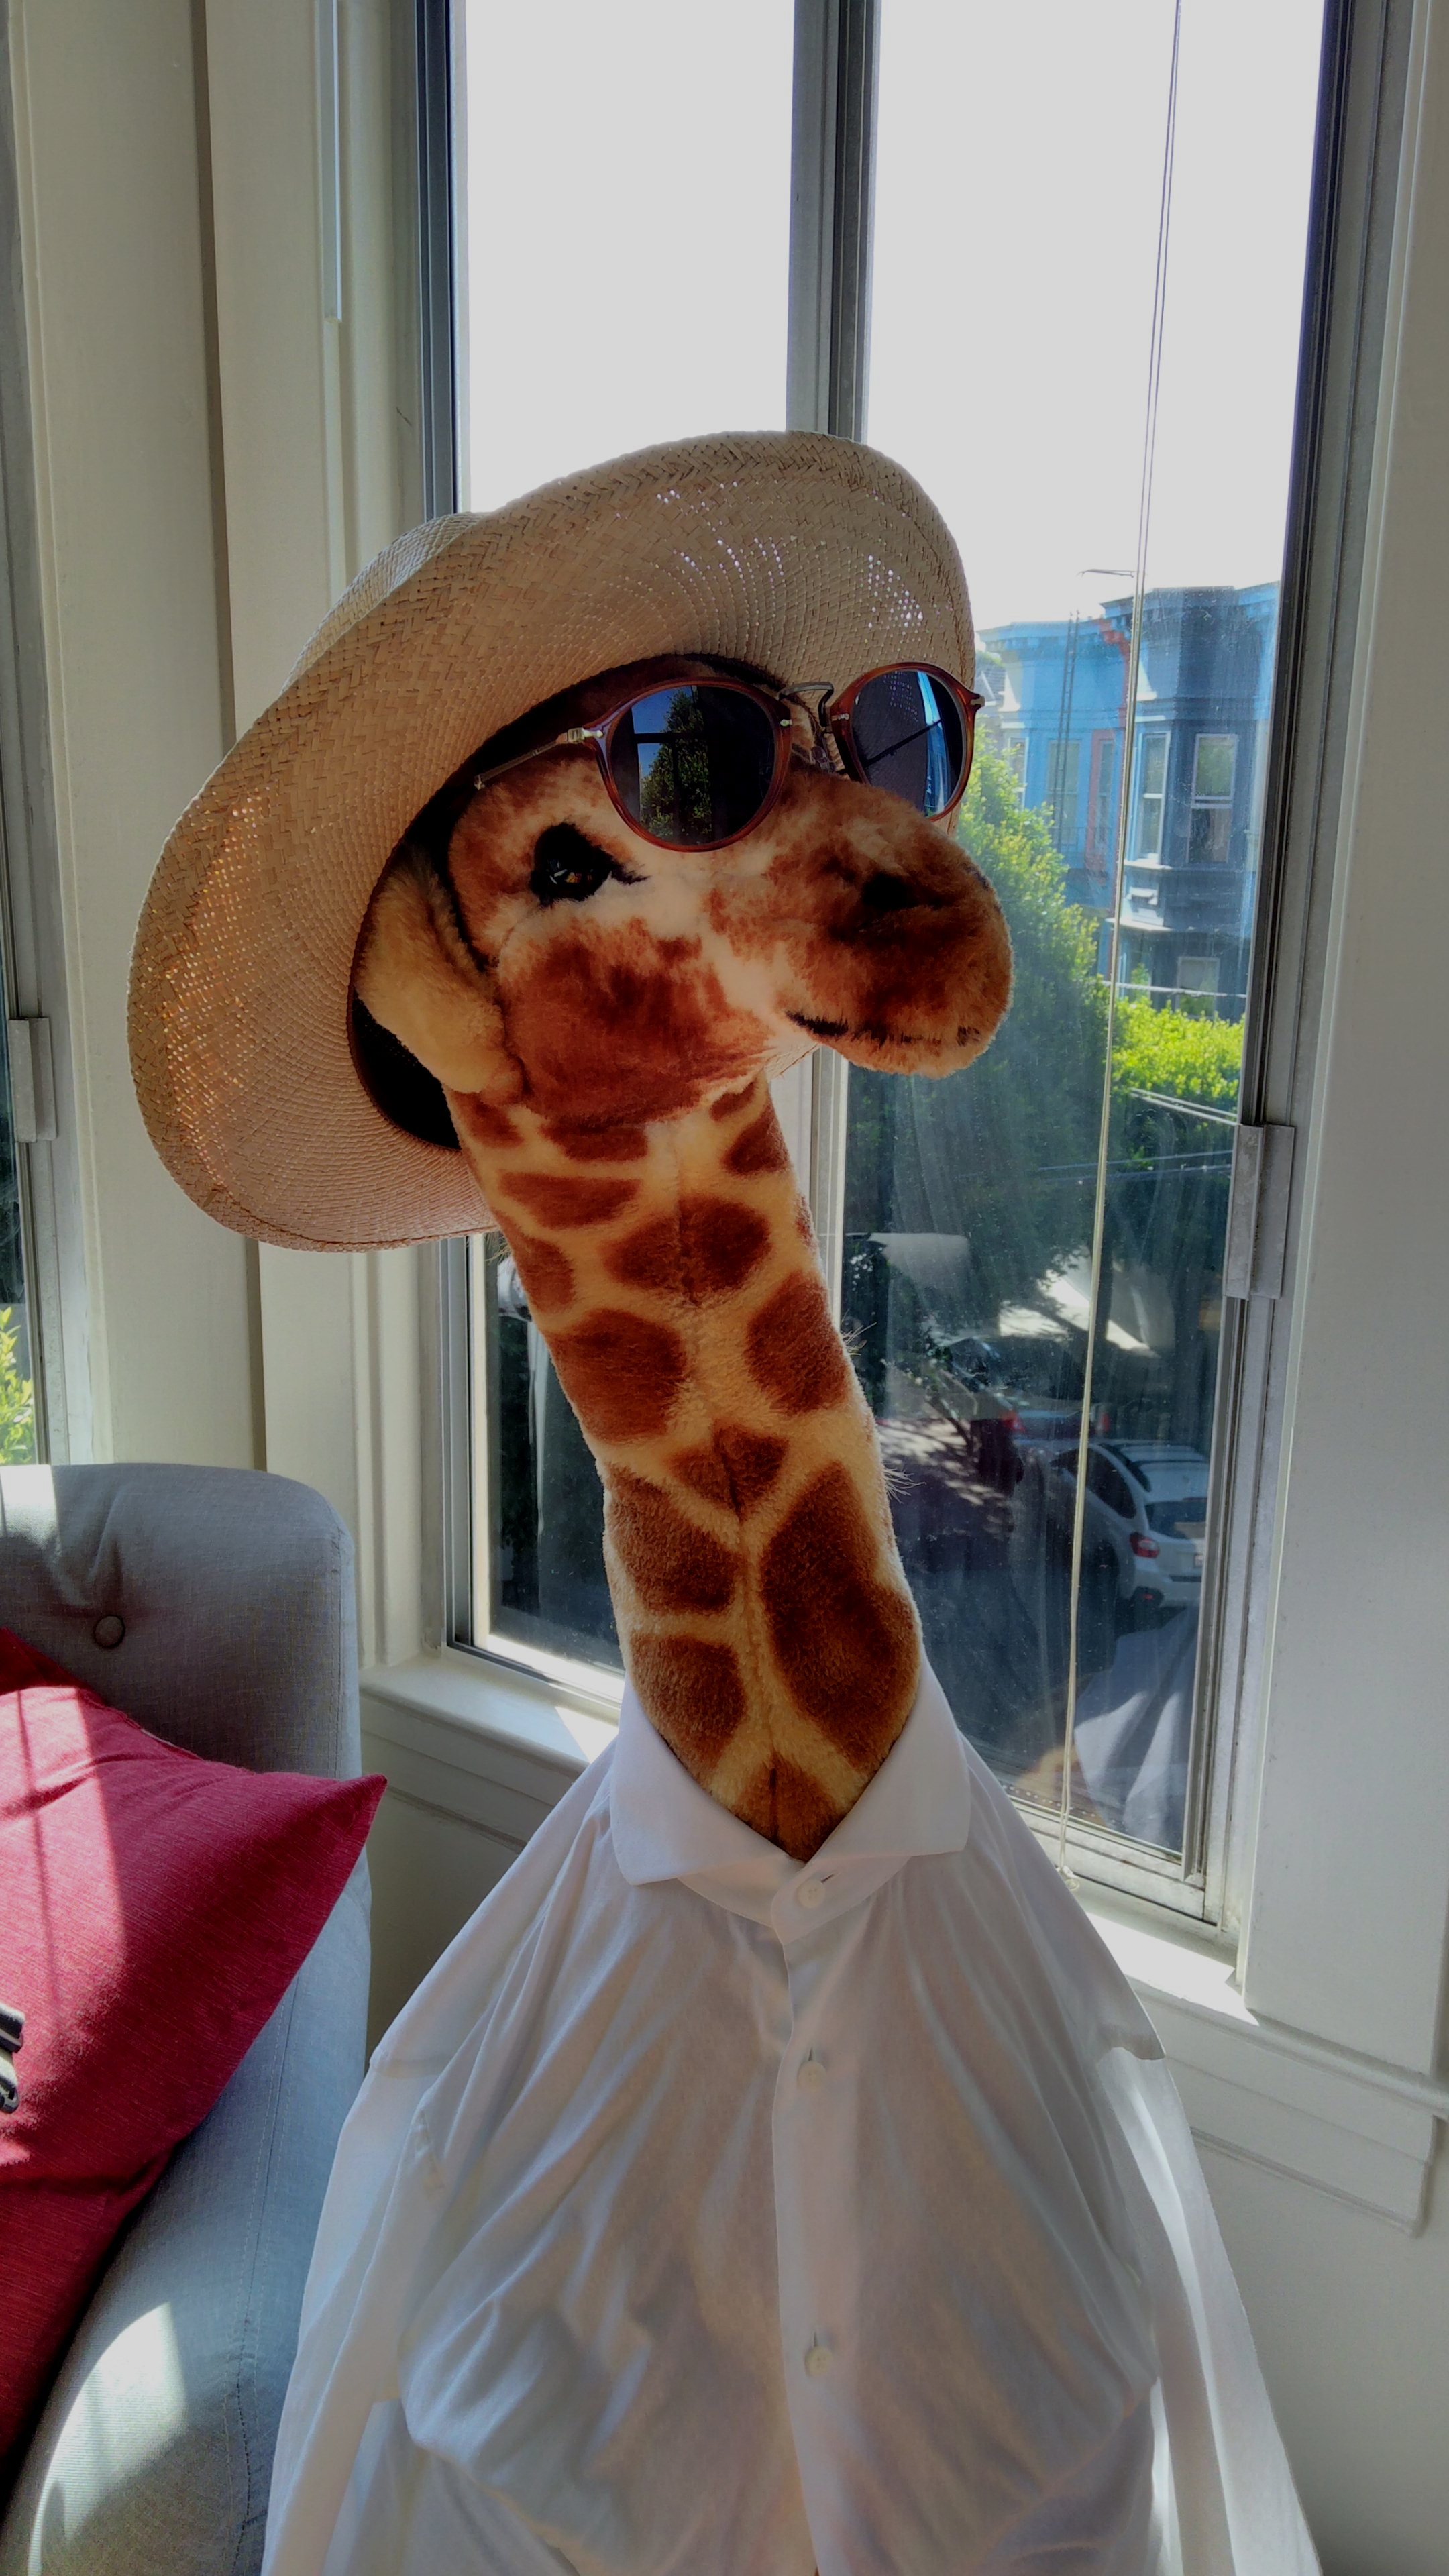
\includegraphics[width=15cm]{result.png}
		\label{fig:result1}
	\end{figure}
	
	
	
	%%%%%%%%%%%%%%%%%%%%%%%%%%%%%%%%%%%
	
	
	% If you really need extra space, uncomment here and use extra pages after the last question.
	% Please refer here in your original answer. Thanks!
	%\pagebreak
	%\paragraph{AX.X Continued:} Your answer continued here.
	
	
	
\end{document}